\documentclass[dvisvgm]{standalone}
\usepackage{tikz}
\usetikzlibrary{shapes,arrows, positioning,fit}

\begin{document}
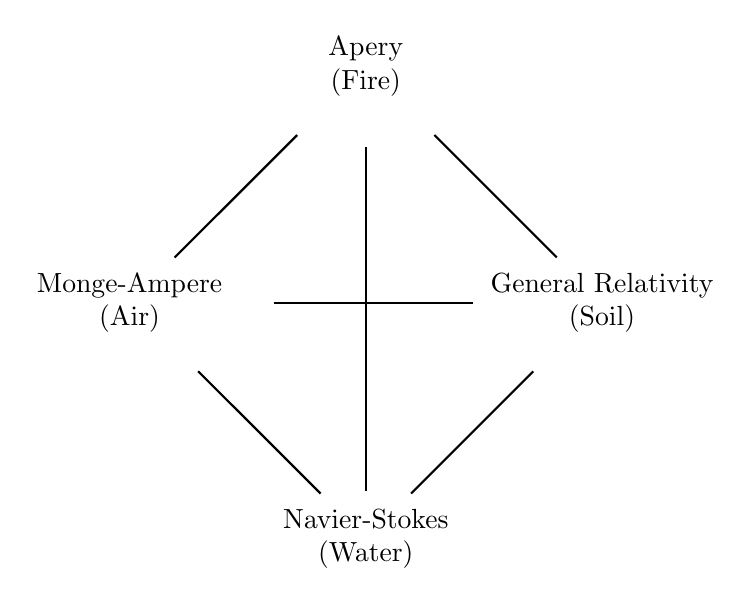
\begin{tikzpicture}[auto, every node/.style={align=center}]
  \node (a) at ( 3, 6) {Apery\\(Fire)};
  \node (b) at ( 0, 3) {Monge-Ampere\\(Air)};
  \node (c) at ( 6, 3) {General Relativity\\(Soil)};
  \node (d) at ( 3, 0) {Navier-Stokes\\(Water)};
  \draw[-, shorten <= 15pt, shorten >= 3pt, thick] (a)  -- (b);
  \draw[-, shorten <= 15pt, shorten >= 3pt, thick] (a)  -- (c);
  \draw[-, shorten <= 15pt, shorten >= 3pt, thick] (a)  -- (d);
  \draw[-, shorten <= 15pt, shorten >= 3pt, thick] (b)  -- (c);
  \draw[-, shorten <= 15pt, shorten >= 3pt, thick] (b)  -- (d);
  \draw[-, shorten <= 15pt, shorten >= 3pt, thick] (c)  -- (d);
\end{tikzpicture}
\end{document}
